\documentclass{article}
\usepackage{amsmath,amssymb,amsthm}
\newcommand*{\QEDB}{\hfill\ensuremath{\square}}
\newtheorem*{prop}{Proposition}
\renewcommand{\theenumi}{\alph{enumi}}
\usepackage[shortlabels]{enumitem}
\usepackage[nobreak=true]{mdframed}
\usepackage{tikz}
\usetikzlibrary{matrix,calc}
\usepackage{color}
\usepackage{chngpage}
\usepackage{soul}
\usepackage{hyperref}
\usepackage{csquotes}
\MakeOuterQuote{"}
\hypersetup{
    colorlinks=true,
    linkcolor=blue,
    filecolor=magenta,      
    urlcolor=cyan,
}
\urlstyle{same}
\usepackage{graphicx}
\usepackage{floatrow}
\usepackage[margin=0.75in]{geometry}

\title{Problem Set 3}
\author{Name: $\quad$SID: }
\date{Spring 2016$\quad$GSI: }
\begin{document}
\maketitle

\subsection*{1. Homework Process and Study Group}
Who else did you work with on this homework? List names and student ID's. (In case of hw party, you can also just describe the group.) How did you work on this homework? Working in groups of 3-5 will earn credit for your "Sundry" grade.
\begin{mdframed}
\textbf{Solution}
% Solution here

\end{mdframed}

\clearpage

\subsection*{2. Stable Roommates Problem}
Suppose you are the head of the residential assistants in charge of assigning roommates. Currently you have four students who are going to move in: Kevin, Bryan, Jimmy and Michael. They have submitted their application with the following preferences:
\begin{center}
\begin{tabular}{ |c|c| } 
\hline
Kevin & Bryan $>$ Michael $>$ Jimmy \\
Bryan & Jimmy $>$ Kevin $>$ Michael \\
Jimmy & Kevin $>$ Bryan $>$ Michael \\
Michael & Kevin $>$ Bryan $>$ Jimmy \\
\hline
\end{tabular}
\end{center}
Consider an modified propose-and-reject algorithm which consists of each person $x$, one by one, proposing to the first person $y$ on their list and executing as follows:
\begin{itemize}
\item When $y$ is proposed by $x, y$ crosses off everyone below $x$ on $y$'s list.
\item If $y$ holds $2$ proposals, $y$ rejects the person $y$ prefers least (crosses off the person on $y$'s list).
\item When $x$ is rejected by $y, x$ crosses off $y$ on $x$'s list and proposes to the next person immediately.
\end{itemize}
This continues until everyone holds exactly one proposal. We start with the following proposals and produce the following table:
\begin{center}
\begin{tabular}{ l l l } 
Kevin & $\to$ & Bryan, Bryan crosses off Michael \\
Bryan & $\to$ & Jimmy, Jimmy crosses off Michael \\
Jimmy & $\to$ & Kevin \\
Michael & $\to$ & Kevin, Kevin rejects/crosses off Jimmy, Jimmy crosses off Kevin \\
Jimmy & $\to$ & Bryan, Bryan rejects/crosses off Kevin, Kevin crosses off Bryan \\
Kevin & $\to$ & Michael, Michael crosses off Bryan and Jimmy \\
\end{tabular} 
\end{center}
\begin{center}
\begin{tabular}{ |c|c| } 
\hline
Kevin & \st{Bryan} $>$ Michael $>$ \st{Jimmy} \\
Bryan & Jimmy $>$ \st{Kevin} $>$ \st{Michael} \\
Jimmy & \st{Kevin} $>$ Bryan $>$ \st{Michael} \\
Michael & Kevin $>$ \st{Bryan} $>$ \st{Jimmy} \\
\hline
\end{tabular}
\end{center}
Since each person only has a list size of one, the algorithm terminates with the pairing: $$\{(\text{Kevin},\text{Michael}), (\text{Bryan}, \text{Jimmy})\}$$
Now consider there are two more students who want to apply for housing: Joshua and Justin. Try the algorithm on the following table to find a pairing:
\begin{center}
\begin{tabular}{ |c| l l l l l l l l l | } 
\hline
Kevin & Bryan & $>$ & Joshua & $>$ & Michael & $>$ & Jimmy & $>$ & Justin \\
Bryan & Joshua & $>$ & Jimmy & $>$ & Kevin & $>$ & Justin & $>$ & Michael \\
Jimmy & Kevin & $>$ & Joshua & $>$ & Bryan & $>$ &  Michael & $>$ & Justin \\
Michael & Justin & $>$ & Kevin & $>$ & Bryan & $>$ & Jimmy & $>$ & Joshua \\
Joshua & Kevin & $>$ & Justin & $>$ & Bryan & $>$ & Michael & $>$ & Jimmy \\
Justin & Jimmy & $>$ & Michael & $>$ & Joshua & $>$ & Kevin & $>$ & Bryan \\
\hline
\end{tabular}
\end{center}
Note: The output of this example will be a stable pairing. However, for any instance, if it has a stable pairing, the algorithm cannot guarantee to find the stable pairing. In fact, the algorithm described above is only the Phase 1 of the Irving Algorithm. With the Phase 2, the Irving Algorithm can always find a stable pairing, if the given instance has one. For more information, please check \url{https://en.wikipedia.org/wiki/Stable_roommates_problem}
\begin{mdframed}
\textbf{Solution}
% Solution here

\end{mdframed}

\clearpage

\subsection*{3. Induction on Graphs}
What is wrong with the following "proof"?

\vspace{3mm}
\noindent\textbf{False Claim:} If every vertex in an undirected graph has degree at least $1$, then the graph is connected.

\vspace{3mm}
\noindent\textit{Proof:} We use induction on the number of vertices $n\geqslant 1$.

\vspace{3mm}
\noindent\textit{Base case:} There is only one graph with a single vertex and it has degree $0$. Therefore, the base case is vacuously true, since the if-part is false.

\vspace{3mm}
\noindent\textit{Inductive hypothesis:} Assume the claim is true for some $n\geqslant 1$.

\vspace{3mm}
\noindent\textit{Inductive step:} We prove the claim is also true for $n+1$. Consider an undirected graph on $n$ vertices in which every vertex has degree at least $1$. By the inductive hypothesis, this graph is connected. Now add one more vertex $x$ to obtain a graph on $(n+1)$ vertices, as shown below.
\begin{center} 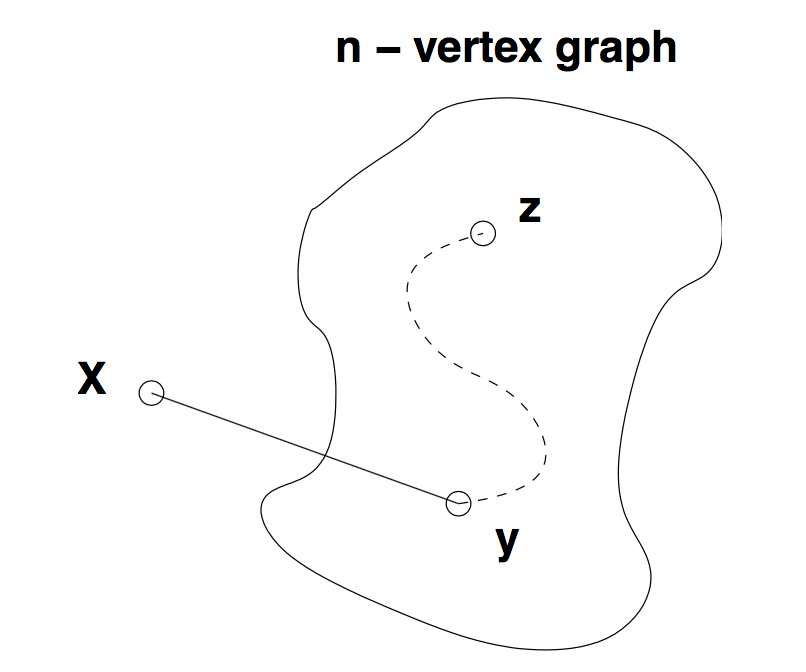
\includegraphics[scale=0.15]{graph.png}\end{center}
All that remains is to check that there is a path from $x$ to every other vertex $z$. Since $x$ has degree at least $1$, there is an edge from $x$ to some other vertex; call it $y$. Thus, we can obtain a path from $x$ to $z$ by adjoining the edge $\{x, y\}$ to the path from $y$ to $z$. This proves the claim for $n+1$. 

\QEDB
\begin{mdframed}
\textbf{Solution}
% Solution here

\end{mdframed}

\clearpage

\subsection*{4. Graphs}
\begin{enumerate}
\item Suppose we have n websites such that for every pair of websites $A$ and $B$, either $A$ has a link to $B$ or $B$ has a link to $A$. Prove or disprove that there exists a website that is reachable from every other website by clicking at most $2$ links. (\textit{Hint: Induction})
\begin{mdframed}
\textbf{Solution}
% Solution here

\end{mdframed}
\item We have shown in the lecture (or you have read Lecture Note 5) that a connected undirected graph has an Eulerian tour if and only if every vertex has even degree. 

Prove or disprove that if a connected graph $G$ on $n$ vertices has exactly $2d$ vertices of odd degree, then there are $d$ walks that \textit{together} cover all the edges of $G$ (i.e., each edge of $G$ occurs in exactly one of the $d$ walks; and each of the walks should not contain any particular edge more than once).
\begin{mdframed}
\textbf{Solution}
% Solution here

\end{mdframed}
\end{enumerate}
\clearpage

\subsection*{5. Another Problem on Graphs}
In this problem, we are given a bipartite graph: $G=(L,R,E)$ where there are two sets of vertices, $L$ and $R$, and $E\subseteq L\times R$, or each edge is incident to a vertex in $L$ and a vertex in $R$. We also know that every vertex has degree \textit{exactly} $d$.

We wish to partition the edges into $d$ perfect matchings: a perfect matching is a set of edges where every vertex is incident to exactly one edge in the matching. Another view is that each vertex is matched to another vertex; similar to a pairing in stable marriage except that the pair must correspond to an edge in the graph. A matching is a set of edges where the number of edges incident to any vertex is at most $1$ (as opposed to equal to $1$ for a perfect matching.)
\begin{enumerate}
\item Draw a $6$ vertex example graph that for $d=2$ that meets the conditions above for an instance.
\begin{mdframed}
\textbf{Solution}
% Solution here

\end{mdframed}
\item Indicate two matchings in your graph that cover the edges.
\begin{mdframed}
\textbf{Solution}
% Solution here

\end{mdframed}
\item Prove that for any instance of this problem that $|L|=|R|$. (Remember every vertex has degree $d$ for any instance.)
\begin{mdframed}
\textbf{Solution}
% Solution here

\end{mdframed}
\item Prove that the length of any cycle in an instance of this problem is even.
\begin{mdframed}
\textbf{Solution}
% Solution here

\end{mdframed}
\item Prove that you can partition the edges in a simple cycle in this graph into exactly two perfect matchings with respect to the vertices in the cycle.
\begin{mdframed}
\textbf{Solution}
% Solution here

\end{mdframed}
\item Assume $d$ is a power of $2$; $d=2^k$ for some natural number $k$. Give an efficient algorithm to compute a partition of the edges into perfect matchings. (Note that trying all possible partitions is not efficient. The algorithm should not take exponential time.)
\begin{mdframed}
\textbf{Solution}
% Solution here

\end{mdframed}
\item Prove your algorithm from the previous part is correct.
\begin{mdframed}
\textbf{Solution}
% Solution here

\end{mdframed}
\end{enumerate}

\clearpage

\subsection*{6. Trees}
Show that the edges of a complete graph on $n$ vertices for even $n$ can be partitioned into $\frac n2$ edge disjoint spanning trees.

\noindent Recall that a complete graph is an undirected graph with an edge between every pair of vertices. The complete graph has $\frac{n(n-1)}{2}$ edges. A spanning tree is a tree on all $n$ vertices --- so it has $n-1$ edges. So the complete graph has enough edges (for even $n$) to create $\frac n2$ edge disjoint spanning trees (i.e. each edge participates in exactly one spanning tree). You have to show that this is always possible.
\begin{mdframed}
\textbf{Solution}
% Solution here

\end{mdframed}
\clearpage

\subsection*{7. Another Problem on Trees}
Recall that a \textbf{tree} is a connected acyclic graph (graph without cycles). In the note, we presented a few other definitions of a tree, and in this problem, we will prove two fundamental properties of a tree, and derive two definitions of a tree we learn from lecture note based on these properties. Let's start with the properties:
\begin{enumerate}
\item  Prove that any pair of vertices in a tree are connected by exactly one (simple) path.
\begin{mdframed}
\textbf{Solution}
% Solution here

\end{mdframed}
\item Prove that adding any edge to a tree creates a simple cycle.
\begin{mdframed}
\textbf{Solution}
% Solution here

\end{mdframed}

\begin{adjustwidth}{-0.35in}{} Now you will show that if a graph satisfies either of these two properties then it must be a tree: \end{adjustwidth}

\item Prove that if every pair of vertices in a graph are connected by exactly one simple path, then the graph must be a tree.
\begin{mdframed}
\textbf{Solution}
% Solution here

\end{mdframed}
\item  Prove that if the graph has no simple cycles and has the property that the addition of any single edge (not already in the graph) will create a simple cycle, then the graph is a tree.
\begin{mdframed}
\textbf{Solution}
% Solution here

\end{mdframed}
\end{enumerate}

\clearpage

\subsection*{8. Hypercubes}
\begin{enumerate}
\item Prove that any cycle in an $n$-dimensional hypercube must have even length.

\noindent Recall that a cycle is a closed (simple) path and its length is the number of vertices (edges) in it. The $n$ dimensional hypercube is a graph whose vertex set is the set of $n$-bit strings, with an edge between vertices $u$,$v$ iff they differ in exactly one bit (Hamming distance $=1$).
\begin{mdframed}
\textbf{Solution}
% Solution here

\end{mdframed}
\item A \textit{Hamiltonian path} in an undirected graph $G=(V,E)$ is a path that goes through every vertex \textit{exactly once}. A \textit{Hamiltonian cycle} (or \textit{Hamiltonian tour}) is a cycle that goes through every vertex exactly once. Note that, in a graph with $n$ vertices, a Hamiltonian path consists of $n-1$ edges, and a Hamiltonian cycle consists of $n$ edges.

\noindent Prove that for every $n\geqslant 2$, the $n$-dimensional hypercube has a Hamiltonian cycle.
\begin{mdframed}
\textbf{Solution}
% Solution here

\end{mdframed}
\end{enumerate}
\clearpage

\subsection*{9. Four Colorable?}
In the lecture, we have shown that every planar graph can be colored with five colors. We have also shown that it can also be colored with only four colors. The coloring example of U.S. map is shown below. In this question, prove the following: any planar graph of maximum degree $4$ has a four coloring.

\begin{figure}[!h]
\centering
\begin{minipage}{.5\textwidth}
  \centering
  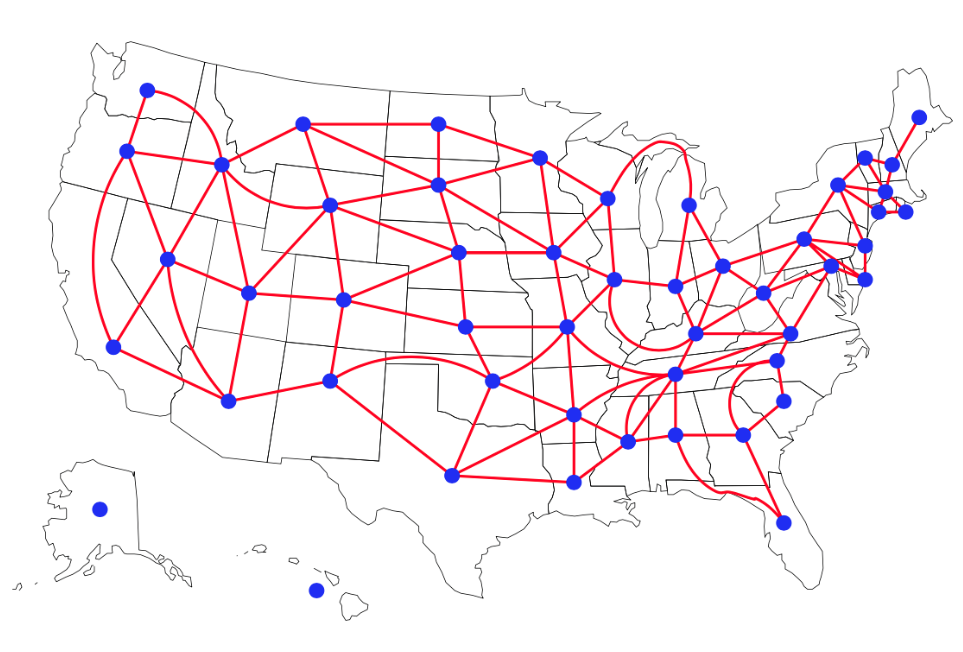
\includegraphics[width=.4\linewidth]{usa0.png}
\end{minipage}%
\begin{minipage}{.5\textwidth}
  \centering
  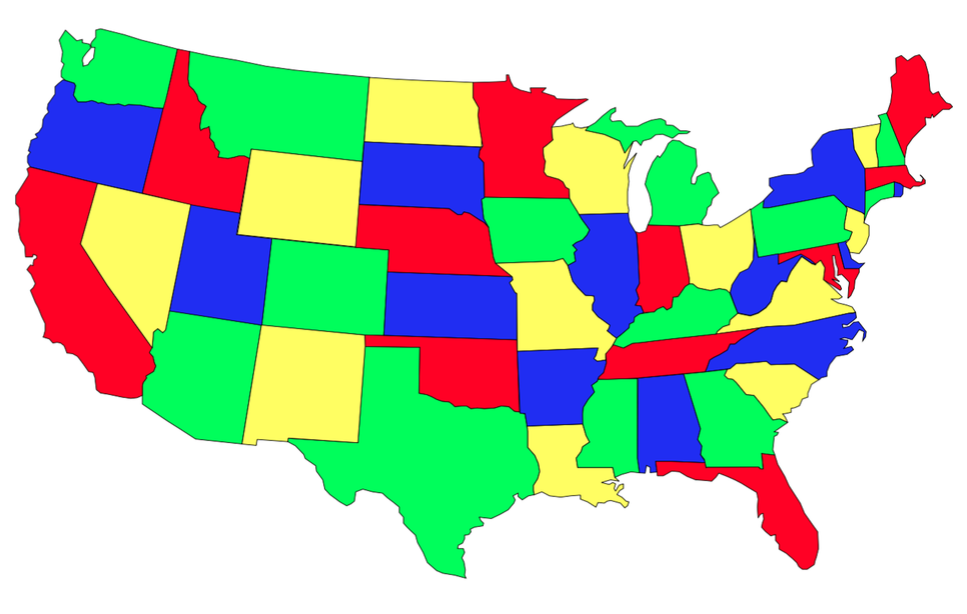
\includegraphics[width=.4\linewidth]{usa1.png}
\end{minipage}
\end{figure}

\begin{mdframed}
\textbf{Solution}
% Solution here

\end{mdframed}
\clearpage


\end{document}